\documentclass[11pt]{article}
\usepackage{../../cs70}
%\usepackage{../../markup}
\usepackage{color}
%\usepackage{amssymb, amsfonts, amsmath, textcomp}
\newif\ifsolutions
\solutionstrue
%\solutionsfalse %flag for solutions
\def\title{Homework 3}

\renewcommand{\answer}[1]{{\color{mydarkblue}\textbf{Solutions: }#1}}
\definecolor{mydarkblue}{rgb}{0,0.25,1}


\begin{document}
\maketitle

\vspace{0.5em}
{\Large{\textbf{This homework GRADE is due Feb 17 2014, at 12:00 noon.}}}


\begin{qunlist}

\qns{The War with the Four-headed Dragon} \\ 
In this problem, we will consider an ongoing war between ninjas and a massive four-headed dragon. 
The four heads of the dragon are fair to each other: 
they will only eat if each of them have an equal share. One of the heads is compassionate. 
Therefore when the number of ninjas is divisible by 4, the dragons begin eating.  
One fourth of the ninjas live on under the compassionate head, 
but the remaining three fourths of the warriors are eaten. 
If there are an even number of ninjas, and the dragons aren't eating 
(the number is not divisible by four), then two ninjas sneak onto the battle field. 
(The dragon begin eating when again the number of ninjas is divisible by 4.)
When there is an odd number of ninjas, the ninjas see this as their time to pounce. 
Each ninjas summons two of her ninja friends to join the battle, 
thus the number of ninjas is multiplied by three. 
However, exactly one ninja fails to answer the call of battle each time. 
When there is only one ninja left on the battle field, the ninja flees. 
Prove that all battles (no matter how many ninjas initially start fighting) 
end with the ninja fleeing. \\
You can represent this battle by repeatedly applying the following function:
\[ f(n) = \left\{ 
    \begin{array}{cl} 
        n/4 & \text{if $n$ is divisible by 4} \\
        (n+2)/4 & \text{if $n$ is even but not divisible by 4} \\
        3n - 1 & \text{if $n$ is odd} 
    \end{array} 
\right. \]

\textit{Mathematical aside: This problem is reminiscent of the Collatz Conjecture, which you may find interesting. Looking up the Colllatz Conjecture is not necessary for this homework.}

\ifsolutions
\answer{
We want to prove that for any natural number $n$, repeatedly applying $f(n)$ will eventually yield $1$. 
Call this property $P(n)$. We can prove $P(n), \forall n \in \mathbb{N}$ by strong induction.

\underline{Base case:} If $n=1$, we have reached $1$, so $P(1)$ holds.

\underline{Inductive hypothesis:} We assume that for $1 \leq k \leq n$, 
$P(k)$ holds (strong inductive hypotheses).

\underline{Inductive step:} Now we want to show that $P(n+1)$ holds. There are three cases:
\begin{itemize}
\item $n+1$ is divisible by 4: In this case $f(n+1) = (n+1)/4$. 
Since 
\[ \frac{n+1}{4} = \frac{n}{4} + \frac{1}{4} < n+1, \quad \forall n \geq 1, \]
we have reached a number strictly less than $n+1$. We also know that  $(n+1)/4$ is a natural number because $n$ is divisible by $4$. So by our inductive hypothesis $P(f(n+1))$ holds, which implies $P(n+1)$.
\item $n+1$ is even but not divisible by 4: In this case $f(n+1) = (n+3)/4$. 
Since 
\[ \frac{n+3}{4} = \frac{n}{4} + \frac{3}{4} < n+1, \quad \forall n > 1, \]
we have reached a number strictly less than $n+1$. We argue that this number must be a natural number because if $n+1$ is even but not divisible by four, then $n+3$ must be divisible by four. This is because $n+1 = 4k + 2$ for some k, since it is even but not divisible by $4$, it must be two greater than a multiple of $4$. Therefore, $n + 1 + 2 = 4k + 2 + 2 = 4(k+1)$ which is of course divisible by four. So, $(n+3)/4$ is a natural number less than $n+1$ So by our inductive hypothesis $P(f(n+1))$ holds, which implies $P(n+1)$.
\item $n+1$ is odd: In this case $f(n+1) = 3(n+1) - 1$, which will be even.  
So then we can apply $f$ again to reduce it to a problem we have already solved.  
Then $f(f(n+1)) = (3n+2)/4$ or $f(f(n+1)) = (3n+4)/4$. Since
\[ \frac{3n+4}{4} = \frac{3}{4} n + 1 < n+1, \quad \forall n\geq 1, \]
both of these options are strictly less than $n+1$. Also, both of these numbers will be natural numbers for the same reasons specified in the earlier cases.
Therefore by our inductive hypothesis, $P(f(f(n+1)))$ holds, which implies $P(n+1)$.
\end{itemize}
}
\fi

\pagebreak

\qns{Make it stronger again} \\
Define the following sequence: $a_1 =2$, $a_2 = 3$ and $a_k = a_{k-1} \cdot a_{k-2}$ for all $k \geq 3$. \\ 
Does the sum 
\[ A_n = \sum_{k=1}^n \frac{1}{a_k} \]

diverge (i.e. approach infinity) as $n \to \infty$, or does it converge to a finite number?  
Prove why or why not.
{\em Hint: plot $A_n$ and think about discussion 2B.}

\ifsolutions
\answer{
It does converge. We can prove this by comparing this series with a series of which the behavior is known: 
a geometric series. We will use the fact that
\[ 1 + r + r^2 + r^3 + \cdots = \sum_{k=1}^{\infty} r^{k-1} = \frac{1}{1-r}, \quad \text{for } |r| < 1, \]

which means that for $|r| < 1$, the sum of this series converges to a finite number. 
So if we can show that the sum of our series is less than the sum of a geometric series, 
then our series also converges. We will use the geometric series in the case when $r = 1/2$.
To prove that each term of our series is less than the corresponding term in the geometric series, 
we can use strong induction to show:
\[ \frac{1}{a_k} < \frac{1}{2^{k-1}}, \quad \text{for all } k \geq 1 \]

\underline{Base cases:} For $k=1$ and $k=2$, 
\[ 
\frac{1}{a_1} = \frac{1}{2} < 1, \qquad 
\frac{1}{a_2} = \frac{1}{3} < \frac{1}{2} 
\]

\underline{Inductive hypothesis:} We assume that 
\[ \frac{1}{a_j} < \frac{1}{2^{j-1}}, \quad \text{for all $j$, } 1 \leq j \leq k \]

\underline{Inductive step:} To get to $k+1$, we can use the recursive definition of our series:
\[ 
\frac{1}{a_{k+1}} = \frac{1}{a_k \cdot a_{k-1}} 
< \frac{1}{2^{k-1} \cdot 2^{k-2}} = \frac{1}{2^{2k-3}} 
\leq \frac{1}{2^k}, \quad \text{for } k > 2 
\]

Since we have proved that each term of our series is smaller than 
the corresponding term of this geometric series, then the sum of our series must be smaller as well:
\[ \sum_{k=1}^{\infty} \frac{1}{a_k} < \sum_{k=1}^{\infty} \frac{1}{2^{k-1}} = 2 \]

Therefore, since sum of the geometric series converges, the sum of our series at least does not diverge. One possibility is that the sum oscillates, so it doesn't converge, but is still bounded. In our case though, all the $a_n$ terms are positive, so the sum is monotonically increasing. Therefore it must not oscillate, and thus converges to a finite number.
}
\fi


%\qns{backup prob} \\
%Let $x,y$ be real numbers such that the numbers $x+y$, $x^2+y^2$, $x^3+y^3$, and $x^4+y^4$ are integers. \\ 
%Prove that for all positive integers $n$, the number $x^n + y^n$ is an integer.
%
%\ifsolutions
%\textbf{Solutions:}
%Use strong induction. Use the identity
%\[ x^{k+1} + y^{k+1} = (x+y)(x^k + y^k) - xy(x^{k-1} + y^{k-1}) \]
%
%We are given that $x+y$ is an integer, and by our inductive hypothesis $x^k + y^k$ and $x^{k-1} + y^{k-1}$ 
%are also both integers. So we need to show that $xy$ is an integer.  This can be shown because:
%\[ x^3 + y^3 = (x+y)(x^2+y^2) - xy(x+y) \]
%
%So our base cases are $n=5$ and $n=6$.  After that we can use strong induction.
%\fi


\pagebreak

\qns{A tiling problem} \\
You are given three kinds of tiles, \textbf{A,B,C} of dimensions $1 \times 2$, $2 \times 1$
and $2 \times 2$ respectively (as shown in the figure below).
\textit{Note that rotations of the tiles are not allowed, so tiles \textbf{A} and \textbf{B} are NOT the same!}

\begin{minipage}{\linewidth}
\centering
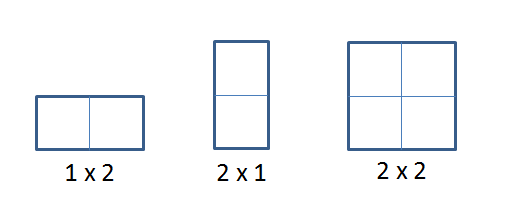
\includegraphics[scale=0.6]{resources/figures/tile.png}
\end{minipage}

Your goal is to tile a board of dimension $2 \times n$, and you are interested in the number of
tiling configurations possible using the three types of tiles given. \\
Let $T_n$ denote the number of tiling configurations for a board of dimension $2 \times n$.
\begin{itemize}
\item[(a)] As preparation for the inductive steps, derive the relations between $T_n$, $T_{n-1}$ 
and $T_{n-2}$ for all $n \geq 3$. \textit{Hint: compute $T_n$ by direct enumeration for small $n$'s.}

\ifsolutions
\answer{
\[ T_n = T_{n-1} + 2T_{n-2}, \quad \text{for all } n \geq 3 \]
We enumerate the tilings for a $2 \times n$ board by considering three cases depending on
the type of tile covering the bottom square of the first column. 
\begin{itemize}
\item[(i)] The tile is of type \textbf{A}: 
then the first two columns of the board must be tiled with \textbf{AA}.
The remaining $2 \times (n-2)$ board can be tiled in $T_{n-2}$ ways.
\item[(ii)] The tile is of type \textbf{B}: the first column is tiled with \textbf{B}, and
the remaining $2 \times (n-1)$ board can be tiled in $T_{n-1}$ ways.
\item[(iii)] The tile is of type \textbf{C}: the first two columns of the board are tiled with \textbf{C}, 
and the remaining $2 \times (n-2)$ board can be tiled in $T_{n-2}$ ways.
\end{itemize}
Note that the three cases are exhaustive and mutually exclusive. The number of tilings for a $2 \times n$
board therefore satisfies the recurrence relation as proposed.
}
\fi


\newpage

\item[(b)] Prove by induction that for all $n \geq 1$
\[ T_n = \frac{2^{n+1}+(-1)^n}{3} \]

\ifsolutions
\answer{
(Strong Induction) $P(n=k)$ asserts that $T_k = \frac{2^{k+1}+(-1)^k}{3}$. 
We prove the statement by (strong) induction on $k$, showing that $P(k-2) \wedge P(k-1) \implies P(k)$.

\underline{Base cases:} $T_1 = 1$ as there is exactly one way to tile a $2 \times 1$ board, 
using tile \textbf{B}.
The $2 \times 2$ board can be tiled in exactly three different ways 
using the tiles \textbf{AA, BB} and \textbf{C},
so $T_2 = 3$. The base cases are true as 
\[P(1)=T_1=1=\frac{2^2+(-1)}{3} \quad\quad\quad P(2)=T_2=3=\frac{2^3+1}{3}\]

\underline{Induction Hypothesis:} Assume $P(k-1)$ and $P(k-2)$ are true for all $n=k > 2$.

\underline{Inductive step:} Using the recurrence relation derived in part (a), we have,
\begin{align*} 
T_k &= T_{k-1} + 2T_{k-2} \\
&= \frac{2^k + (-1)^{k-1}}{3}+2\cdot\frac{2^{k-1}+(-1)^{k-2}}{3}  &\text{[by induction hypothesis]} \\
&= \frac{2\cdot 2^k+(-1)^{k-2}(-1+2)}{3} \\
&= \frac{2^{k+1}+(-1)^k}{3}  &\text{[as } (-1)^{k-2} = (-1)^k \text{]} \\
\end{align*}
The claim is therefore true by (strong) induction for all natural numbers $n=k \geq 1$.
}
\fi


\end{itemize}



\pagebreak

\qns{Let's grade proofs!} \\
For each of the induction ``proofs'' below, say whether you think the proof is correct or not.
If you think the proof is incorrect, 
explain \textit{clearly} and \textit{concisely} where the logical error lies.
If you think the proof is correct, you do not need to give any explanation. \\
\textit{Recall that simply saying the inductive hypothesis is false is not a valid explanation.}

\begin{itemize}
\item[(a)] \textbf{Claim:} $\forall n \in \N$ , $n^2 \leq n$. \\
\textbf{Proof:} \\
\textit{Base case:} for $n = 1$, the claim is $1^2 \leq 1$, which is true. \\
\textit{Induction hypothesis:} Assume that $k^2 \leq k$. \\
\textit{Inductive step:} We need to show that 
\[ (k+1)^2 \leq k+1\]
Working backwards we see that 
\[ k^2 \leq (k+1)^2 - 1 \leq (k+1) - 1 = k \]
So we get back to our original hypothesis which is assumed to be true.\\
Hence, for every $n \in \N$, we know that $n^2 \leq n$. 

\ifsolutions
\answer{
The claim is clearly false as $2^2 > 2$, so the proof must be incorrect.\\
The base case and the induction hypothesis do not have any errors. The flaw lies in the inductive step.
In fact, working backwards, the proof \textit{implicitly} assumes that $(k+1)^2 \leq k+1$.
But this is what we are trying to prove, we cannot assume it!
}
\fi


\item[(b)]\textbf{Claim:} $\forall n \in \N$ , $7^n = 1$. \\
\textbf{Proof:} \\
\textit{Base case:} Certainly $7^0 = 1$. \\
\textit{Induction hypothesis:} Assume that $7^j = 1$ for all $0\leq j \leq k$.\\
\textit{Inductive step:} We need to prove that $7^{k+1} = 1$, and we have,
\[ 7^{k+1} = \frac{7^k \cdot 7^k}{7^{k-1}} = \frac{1 \cdot 1}{1} = 1\]
Hence, by the Principle of Strong Induction, $7^n = 1$ for all $n \in \N$.

\ifsolutions
\answer{
The claim is clearly false as $7 \ne 1$, so there must be an error in the proof.
The (strong) induction hypothesis is stated correctly, however, not all required base cases are checked.
The inductive step uses both $P(k)$ and $P(k-1)$ to prove $P(k+1)$, which breaks down for $k=0$.
When $k=0$, $k-1 = -1$ and $P(k-1)=P(-1)$ is not defined!
}
\fi

% backup
%\item[(c)]\textbf{Claim:} $\forall n \in \N$, if $n \geq 4$, then $2^n < n!$. \\
%\textbf{Proof:} \\
%Base case: $2^4 = 16$ and $4! = 24$, so the claim is true for $n=4$. \\
%Induction hypothesis: Assume $n \geq 4$ and $2^n < n!$. \\
%Inductive step: \[ 2^{n+1} = 2(2^n) < 2(n!) < (n+1)(n!) = (n+1)!\]
%So we have shown that $2^{n+1} < (n+1)!$ and this completes the proof.
%\ifsolutions
%\textbf{Solutions:} This proof is correct.
%\fi


\item[(c)]\textbf{Claim:} $\forall x,y,n \in \N$, if $\max(x,y) = n$, then $x \leq y$. \\
\textbf{Proof:} \\
\textit{Base case:} For $n=0$, if $\max(x,y) = 0$ and $x,y \in \N$, then $x=0, y=0$, hence $x \leq y$. \\
\textit{Induction hypothesis:} Assume that whenever we have $\max(x,y) = n$, $x \leq y$ must hold. \\
\textit{Inductive step:} We must prove that if $\max(x,y) = n+1$, then $x \leq y$. \\
Suppose $x,y$ are such that $\max(x,y) = n+1$, then it follows that $\max(x-1,y-1) = n$. \\
So by the inductive hypothesis, $x-1 \leq y-1  \implies x \leq y$, completing the proof.

\ifsolutions
\answer{
This proof is incorrect. The use of $\max(x-1, y-1)$ is not correct, 
since $x-1$ and $y-1$ will be negative when $x=0$ or $y=0$.
Then the inductive hypothesis no longer applies, since $x-1$ and $y-1$ 
fall outside the range of natural numbers. We cannot conclude that $x-1 \leq y-1$ and the proof fails.
}
\fi


\end{itemize}


\newpage

\qns{Marty's Marriage Mistake}
\begin{itemize}
\item[(a)] My friend Marty and I run a match-making business. 
We receive preference lists from men and women 
and use the same propose-and-reject algorithm you covered in class. 
Marty, being a traditionalist, insists on having the men propose, 
while I, in a subtle attempt to subvert the patriarchy, have the women propose. 
Prove that if both Marty and I come up with the same pairings, there is no other possible stable pairing 
(i.e. a pairing with no rogue pairs).

\ifsolutions
\answer{

We use the fact that the traditional propose-and-reject algorithm is male-optimal (among all stable pairings) and female-pessimal (among all stable pairings). This is proved in the lecture notes. This means that each man receives the best possible woman he could receive under a stable pairing. If we have the pair (M,W) returned by the traditional propose-and-reject algorithm, then for all other stable pairs where we have (M, W*), we know that M must prefer W more than W*. Similarly, female pessimal means if we have the pair (M,W) returned by the traditional propose-and-reject algorithm, then for all other stable pairs where we have (M*, W), we know that W must prefer M* more than M. None of our assumptions use the fact that it is actually men proposing. Therefore, we may claim that the algorithm is proposer-optimal and rejector-pessimal. 
Since Marty and I get the exact same pairing, by Marty's men-proposing and women-rejecting version, the pairing is female-pessimal (among all stable pairing). By my men-rejecting and women-proposing version, the pairing is female-optimal. Therefore the pairing is both female-pessimal and female-optimal. By similar logic, the pairing is both male-optimal and male-pessimal.

Consider a generic pair returned by our algorithm (M,W). We argue by contradiction that there does not exist a stable pairing where W is paired with another man.
Assume there exists a stable pairing where at least one woman is matched with someone different (M*, W). If W prefers M* more than M, then the original pairing (M,W) is not female-optimal among stable pairings, and we have a contradiction. If W prefers M more than M*, then the original pairing (M,W) is not female-pessimal among stable pairings, and we have a contradiction. Therefore W must prefer M equally to M*. Since the algorithm demands each person has a strict ordering among their preferences (there can be no ties of preference), M* must be the same man as M. Therefore, no woman can be paired with a different man in a stable pairing, and therefore there can be no other stable pairings.

Note: This proof depends on a strict ordering among their preferences, if we try to extend the propose-and-reject algorithm to cover the case of equal preferences, then this proof will no longer hold. Consider the number of stable pairs where everyone ranks everyone equally.
}
\fi


\item[(b)] While I'm on vacation, things get a little disorganized. 
Marty loses track of some of the preference lists. 
He is too embarrassed to ask the women for their preferences again. He knows the following preferences:

\begin{center}
\begin{tabular}{|c|ccc|}\hline 
Man&\multicolumn{3}{|c|}{Women}\\\hline 
1&A&B&C\\\hline 
2&C&B&A\\\hline 
3&A&C&B\\\hline
\end{tabular} 
\hspace{2cm}
\begin{tabular}{|c|ccc|}\hline 
Woman&\multicolumn{3}{|c|}{Men}\\\hline 
A&?&?&?\\\hline 
B&1&2&3\\\hline 
C&?&?&?\\\hline
\end{tabular}
\end{center}
   
Marty decides to assume that A and C would have the same preferences as B. 
Show the steps of Marty running the propose-and-reject algorithm (with men proposing). 
Please indicate the final pairing clearly and note how many days it took to reach that pairing.

\ifsolutions
\answer{
\begin{center}
    \begin{tabular}{| l | l | l |}
    \hline
    Days & Women & Proposals \\ \hline
     1 & A & \textcircled{1} 3 \\ 
       & B &  \\ 
       & C & \ 2 \\ \hline
     2 & A & \ 1 \\ 
       & B &  \\ 
       & C & \textcircled{2} 3 \\ \hline
     3 & A & \ 1 \\ 
       & B & \ 3\\ 
       & C & \ 2 \\ \hline
    \end{tabular}
\end{center}
This takes three days, and returns a potentially stable pairing of \{(A,1), (B,3), (C,2)\}.
}
\fi

\newpage
\item[(c)] When I come back from my vacation, Marty explains the previous situation. 
He smugly informs me that none of the couples have switched after he proposed a matching, 
and therefore there are no rogue pairs. 
Because of this, I shouldn't bother running the algorithm having women propose. 
I am not so certain that he is correct. After all, he ran the algorithm on incomplete data. 
I want to convince him that another pairing could exist. 
Show that (without changing any of the known preferences) 
there exists a list of preferences for A and C in which I would pair them differently. 
Remember, in my version, I have the women propose. 
Is it possible to have everyone paired with somebody different? 
Either provide an example, or prove that it's impossible. 

\ifsolutions
\answer{
We attempt to construct a set of preferences such that everyone is paired with somebody different from the stable pairing results in part (b). First, we make some deductions about the preferences of women. If A prefers 3 over 1, we would have the rogue pair (A,3) in Marty's pairing. Therefore, A must prefer 1 over 3. If C prefers 3 over 2, then (C,3) would be a rogue pair in Marty's pairing. Therefore, C must prefer 2 over 3. 
If A prefers 1 the most, then A and 1 would be "soul mates": if either of them were paired with someone else, they would always form a rogue pair with each other. Since we are attempting to construct a completely different set of preferences, we do not want A and 1 to be together. Therefore, we want to make sure A does not prefer 1 the most. Since A prefers 1 over 3, A must rank 1 second in our preference list (which attempts to create new pairings). We use the same logic for C, noting that if C prefers 2 the most, we would have two "soul mates" again. Since we are trying to come up with a new set of preferences, and since C prefers 2 over 3, C must prefer 2 second in our preference list (which attempts to create new pairings)

We can fill out the chart by now.
\begin{center}
\begin{tabular}{|c|ccc|}\hline 
Woman&\multicolumn{3}{|c|}{Men}\\\hline 
A&2&1&3\\\hline 
B&1&2&3\\\hline 
C&1&2&3\\\hline
\end{tabular}
\end{center}

We double check that the propose-and-reject algorithm (with the women proposing) 
results in a different set of preferences:
\begin{center}
    \begin{tabular}{| l | l | l |}
    \hline
    Days & Men & Proposals \\ \hline
     1 & 1 & \textcircled{B} C \\ 
       & 2 & \ A \\ 
       & 3 &  \\ \hline
     2 & 1 & \ B  \\ 
       & 2 &   \ A \textcircled{C} \\ 
       & 3 &  \\ \hline
     3 & 1 & \ B \textcircled{A} \\ 
       & 2 & \ C \\ 
       & 3 & \  \\ \hline
     4 & 1 & \ A \\ 
       & 2 & \ \textcircled{C} B\\ 
       & 3 & \ \\ \hline
     5 & 1 & \ A \\ 
       & 2 & \ C\\ 
       & 3 & \ B \\ \hline
    \end{tabular}
\end{center}
This takes five days, and returns a potentially stable pairing of \{(A,1), (B,3), (C,2)\}.

We attempted to reach a different stable pairing, but this is the exact same stable pairing. We now try to consider if it is possible to construct a pairing where anyone is paired with someone different. We prove that in all stable pairings, C must be paired with 2.

Assume for contradiction that in a stable pairing C is paired with 1. 
Then (1,B) would be a rogue pair. Contradiction!

Now assume for contradiction that C is paired with 3. 
Then, either A is paired with 2 or A is paired with 1. \begin{itemize}
\item[i]If A is paired with 2, then (2,C) is a rogue couple. Remember that based on our logic above, C must prefer 2 over 3 (other wise the original pairing would not be stable). In addition, by the given male preference list, 2 prefers C over A.
\item[ii]If A is paired with 1, then 2 is paired with B.  Then (2,C) is a rogue couple. Remember that by our logic, C prefers 2 over 3. In addition, 2 prefers C over B based on the given male preference list. \end{itemize}


We have now proven that the only other possible stable pairing is 
\{(A,3), (B,1), (C,2)\}.
Therefore it is impossible to have everyone paired with somebody different.

Is the pairing {(A,3), (B,1), (C,2)} stable? We argue that (A,1) must be a rogue pair. If A prefers 1 over 3 then it is a rogue pair. However if A prefers 3 over 1, then the original pairing that Marty gave is not stable (A,3) would be a rogue pair.

A note on this problem, it was ambiguously worded. The problem can be read to imply another stable pairing is possible, when in fact there is no other stable pairing.

}
\fi


%\item[(d)] At the homework party, two of your friends attempt part (c) above. 
%Here is your first friend's work: 
%\begin{center}
%\begin{tabular}{|c|ccc|}\hline 
%Woman&\multicolumn{3}{|c|}{Men}\\\hline 
%A&1&?&?\\\hline 
%B&1&2&3\\\hline 
%C&?&?&?\\\hline
%\end{tabular} 
%\end{center}

%Here is your second friend's work:
%\begin{center}
%\begin{tabular}{|c|ccc|}\hline 
%Woman&\multicolumn{3}{|c|}{Men}\\\hline 
%A&?&?&?\\\hline 
%B&1&2&3\\\hline 
%C&?&3&?\\\hline
%\end{tabular}
%\end{center}
 
%No matter how the rest of the preferences are filled out, these will result in invalid solutions to part (c). 
%Explain why.

%\ifsolutions
%\textbf{Solutions:} The first friend's work is wrong as explained in part (c). 
%If A ranks 1 first, than A and 1 must be together in all stable pairings. 
%This will result in exactly the same pairing as Marty found. This is an invalid solution for part (c). 
%The second friend's work is also wrong. We know that C prefers 2 over 3 (again, see part (c) for details),
%therefore 2 would have to be first on C's preference list. 
%This would also result in the exact same pairing found in part (a). 
%Again, this solution would be invalid for part (c).
%\fi


\end{itemize} 
    



\newpage

        
\qns{All is fair in love and adversaries}

\begin{itemize}
\item[(a)] It turns out that Marty has gotten his fair share of enemies over the years. 
We receive a stable marriage pairing, but one of his rivals has maliciously eliminated some of the preferences:

\begin{center}
\begin{tabular}{|c|ccc|}\hline 
Man&\multicolumn{3}{|c|}{Women}\\\hline 
1&X&A&X\\\hline 
2&X&X&X\\\hline 
3&C&X&X\\\hline
\end{tabular} 
\hspace{2cm}
\begin{tabular}{|c|ccc|}\hline 
Woman&\multicolumn{3}{|c|}{Men}\\\hline 
A&2&1&3\\\hline 
B&X&X&3\\\hline 
C&X&X&3\\\hline
\end{tabular}
\end{center}
        
Luckily, we correctly guess a stable pairing is \{(A,1), (B,2), (C,3)\}. 
List all the possibilities of filling in the missing preferences such that the pairing we guessed is stable.

\ifsolutions
\answer{
First of all, we look at the pairing (C,3) because 3 is C's least favorite. 
We know that in order for there to be no rogue pairs with 3, 
the other men must prefer their current partners to C. 
Then we have 1 prefers A over C and 2 prefers B over C. 
We can now entirely fill out the preferences for Man 1, since C cannot be first:

\begin{center}
\begin{tabular}{|c|ccc|}\hline 
Man&\multicolumn{3}{|c|}{Women}\\\hline 
1&B&A&C\\\hline 
2&X&X&X\\\hline 
3&C&X&X\\\hline
\end{tabular} 
\end{center}

Now, since we know that 1 prefers B the most, in order for (1,B) not to be a rogue pair, 
B must prefer 2 over 1:

\begin{center}
\begin{tabular}{|c|ccc|}\hline 
Woman&\multicolumn{3}{|c|}{Men}\\\hline 
A&2&1&3\\\hline 
B&2&1&3\\\hline 
C&X&X&3\\\hline
\end{tabular}
\end{center}

Also, 2 must prefer C less than B, otherwise (2,C) would be a rogue pair. Why would it be a rogue pair? Remember that C is paired with her worst choice--this means that C will form a rogue pair with any man who prefers C over his current partner.
In addition, 2 must prefer A less than B, otherwise (2,A) would be a rogue pair. 
Therefore 2 must prefer B the most.

\begin{center}
\begin{tabular}{|c|ccc|}\hline 
Man&\multicolumn{3}{|c|}{Women}\\\hline 
1&B&A&C\\\hline 
2&B&X&X\\\hline 
3&C&X&X\\\hline
\end{tabular} 
\end{center}

At this point, we don't have anymore clues to work with. 
With these preference lists, 
no rogue pairs are generated from the initial pairing that was guessed. 
To double check this, you can run the traditional propose-and-reject algorithm 
with the above preferences and we end up with the original pairing. 
So, there are 8 ways to fill out all the possibilities of this:


\begin{center}
\begin{tabular}{|c|ccc|}\hline 
Man&\multicolumn{3}{|c|}{Women}\\\hline 
1&B&A&C\\\hline 
2&B&?&?\\\hline 
3&C&?&?\\\hline
\end{tabular} 
\hspace{2cm}
\begin{tabular}{|c|ccc|}\hline 
Woman&\multicolumn{3}{|c|}{Men}\\\hline 
A&2&1&3\\\hline 
B&2&1&3\\\hline 
C&?&?&3\\\hline
\end{tabular}
\end{center}


Final answer: 

\begin{center}
\begin{tabular}{|c|ccc|}\hline 
Man&\multicolumn{3}{|c|}{Women}\\\hline 
1&B&A&C\\\hline 
2&B&A&C\\\hline 
3&C&B&A\\\hline
\end{tabular} 
\hspace{2cm}
\begin{tabular}{|c|ccc|}\hline 
Woman&\multicolumn{3}{|c|}{Men}\\\hline 
A&2&1&3\\\hline 
B&2&1&3\\\hline 
C&1&2&3\\\hline
\end{tabular}
\end{center}

\begin{center}
\begin{tabular}{|c|ccc|}\hline 
Man&\multicolumn{3}{|c|}{Women}\\\hline 
1&B&A&C\\\hline 
2&B&C&A\\\hline 
3&C&B&A\\\hline
\end{tabular} 
\hspace{2cm}
\begin{tabular}{|c|ccc|}\hline 
Woman&\multicolumn{3}{|c|}{Men}\\\hline 
A&2&1&3\\\hline 
B&2&1&3\\\hline 
C&1&2&3\\\hline
\end{tabular}
\end{center}

\begin{center}
\begin{tabular}{|c|ccc|}\hline 
Man&\multicolumn{3}{|c|}{Women}\\\hline 
1&B&A&C\\\hline 
2&B&A&C\\\hline 
3&C&A&B\\\hline
\end{tabular} 
\hspace{2cm}
\begin{tabular}{|c|ccc|}\hline 
Woman&\multicolumn{3}{|c|}{Men}\\\hline 
A&2&1&3\\\hline 
B&2&1&3\\\hline 
C&1&2&3\\\hline
\end{tabular}
\end{center}

\begin{center}
\begin{tabular}{|c|ccc|}\hline 
Man&\multicolumn{3}{|c|}{Women}\\\hline 
1&B&A&C\\\hline 
2&B&C&A\\\hline 
3&C&A&B\\\hline
\end{tabular} 
\hspace{2cm}
\begin{tabular}{|c|ccc|}\hline 
Woman&\multicolumn{3}{|c|}{Men}\\\hline 
A&2&1&3\\\hline 
B&2&1&3\\\hline 
C&1&2&3\\\hline
\end{tabular}
\end{center}

\begin{center}
\begin{tabular}{|c|ccc|}\hline 
Man&\multicolumn{3}{|c|}{Women}\\\hline 
1&B&A&C\\\hline 
2&B&A&C\\\hline 
3&C&B&A\\\hline
\end{tabular} 
\hspace{2cm}
\begin{tabular}{|c|ccc|}\hline 
Woman&\multicolumn{3}{|c|}{Men}\\\hline 
A&2&1&3\\\hline 
B&2&1&3\\\hline 
C&2&1&3\\\hline
\end{tabular}
\end{center}

\begin{center}
\begin{tabular}{|c|ccc|}\hline 
Man&\multicolumn{3}{|c|}{Women}\\\hline 
1&B&A&C\\\hline 
2&B&C&A\\\hline 
3&C&B&A\\\hline
\end{tabular} 
\hspace{2cm}
\begin{tabular}{|c|ccc|}\hline 
Woman&\multicolumn{3}{|c|}{Men}\\\hline 
A&2&1&3\\\hline 
B&2&1&3\\\hline 
C&2&1&3\\\hline
\end{tabular}
\end{center}

\begin{center}
\begin{tabular}{|c|ccc|}\hline 
Man&\multicolumn{3}{|c|}{Women}\\\hline 
1&B&A&C\\\hline 
2&B&A&C\\\hline 
3&C&A&B\\\hline
\end{tabular} 
\hspace{2cm}
\begin{tabular}{|c|ccc|}\hline 
Woman&\multicolumn{3}{|c|}{Men}\\\hline 
A&2&1&3\\\hline 
B&2&1&3\\\hline 
C&2&1&3\\\hline
\end{tabular}
\end{center}

\begin{center}
\begin{tabular}{|c|ccc|}\hline 
Man&\multicolumn{3}{|c|}{Women}\\\hline 
1&B&A&C\\\hline 
2&B&C&A\\\hline 
3&C&A&B\\\hline
\end{tabular} 
\hspace{2cm}
\begin{tabular}{|c|ccc|}\hline 
Woman&\multicolumn{3}{|c|}{Men}\\\hline 
A&2&1&3\\\hline 
B&2&1&3\\\hline 
C&2&1&3\\\hline
\end{tabular}
\end{center}
}
\fi

\newpage
        
\item[(b)] I begin to suspect that one of Marty's adversaries may have done worse than eliminate preferences. 
Some of the preferences (no matter eliminated or not) may be switched! Marty isn't too worried. 
He says that if the adversary switches the order of only two of the preferences for one person, 
than it's possible our pairing (based on corrupted preferences) will still have no rogue couples. 
Assuming the information we received in part(a) is not corrupted, 
tell us which two preferences can be switched such that after Marty runs the propose-and-reject algorithm, 
he will get a pairing that is stable. 
(You should note it by index. For example, "The adversary switches A's 1st and 3rd preference").

\ifsolutions
\answer{
There are three solutions. 
Either Man 2's 2nd and 3rd preference, Man 3's 2nd and 3rd preference can be switched, 
or Woman C's 1st and 2nd preferences can be switched. 
If any of these three sets of swithes occur, the algorithm will still return no rogue couples. 
This questions is meant as an elaboration on the previous part in order to 
get you to think about how some parts of preference lists 
may not actually affect the outcome of the traditional propose-and-reject algorithm.
}
\fi

        
\item[(c)] I tell Marty that it's possible that even with just two preferences being switched, 
we could get a lot of rogue pairs. For an arbitrary stable marriage instance with $n$ men and $n$ women, 
how many (at most) rogue pairs could be generated 
by an adversary switching the order of two preferences for one person?

\ifsolutions
\answer{
There can be $n-1$ rogue pairs generated. 

We consider by looking at cases separately. 
Let's consider that our adversary switches the preference list of a man, M'. 
We argue that all rogue couples must involve M'.
We consider the man, M, whose preference list is NOT switched by the adversary. 
M is matched with some W at the end of the algorithm, (M,W). 
Suppose towards contradiction that M prefers some W* to his current partner W. 
We will argue that W* prefers her final M* partner to M, so that (M,W*) cannot be a rogue couple.  Since W* occurs before W in M's list, and since his preference list is not switched, 
he must have proposed to W* before he proposed to W. 
Therefore, according to the algorithm, W* must have rejected M for somebody she prefers. 
By the Improvement Lemma, W* likes her final partner M* at least as much, and therefore prefers him to M.
Thus no man M whose preference list has not been switched can be involved in a rogue couple. 
Since M' is currently matched with one woman, there are at most $n-1$ possible rogue pairs with M'. 
At the end of this proof, we will demonstrate how to construct such a situation. 

Next, we consider that the adversary switches the preference list of a woman, W'. 
We similarly argue that all rogue couples must involve W'. 
We consider the woman, W, whose preference list is not switched by the adversary. 
W is matched with some M at the end of the algorithm, (M,W). 
Suppose towards contradiction we have a rogue couple such that W prefers some M* 
to her current partner and M* prefers W over his current partner.  
If M* prefers W over his current partner, 
then he must have proposed to W before he proposed to his current partner. 
Since W's preferencess have not been switched, then the Improvement Lemma holds. 
Therefore, W must prefer her current partner at least as much as M*. 
This contradicts the assumption of there existing a rogue couple with W (M*, W). 
Therefore, only W' can be involved in rogue couples. 
Again, this indicates a maximum of $n-1$ possible rogue couples.

We now demonstrate one way to achieve this maximum of $n-1$ possible rogue couples. 
If every man ranks the women identically and every women ranks the men identically, 
the adversary can achieve the most damage 
by switching the first and last preference of the most-desired man or the most-desired woman. 
Since this person is the most desired, he/she will end up with the person on the top of his/her list. 
Since the adversary has manipulated his/her list, this person is now actually with his/her least preference. 
Therefore he/she prefers all other possible partners, 
and because he/she is the most desirable, all other possible partners desire him/her. 
Therefore we have $n-1$ rogue couples.
}
\fi


\newpage

\item[(d)] Marty counters by suggesting some preferences are very stable. 
If an hyper-intelligent adversary looks at one person's preference list 
and switches it around to do the most damage possible, 
what are the least number of rogue pairs that will be generated? 
For a Stable Marriage problem with $n$ men and $n$ women, describe these adversary-resistant preferences.

\ifsolutions
\answer{
It's possible that this can generate 0 rogue couples. 

In order for this to happen, create a list of men and women such that 
each pair ranks the other person number one on their preference list. 
We argue that if a man and a woman rank each other as highest preference 
(they are "soul mates"), 
they must be paired together in all stable pairings.
[Assume for contradiction that M and W who rank each other number one 
are paired with other people (M,W*) and (M*,W). 
If this is the case, (M,W) would be a rogue couple because they are both each other's top preference.] 
When the adversary disrupts the preference list of one person, 
we just proved that the other $n-1$ men and $n-1$ women must be paired with their ``soul mates''. 
There is only one way to pair the remaining man and woman (one of whose list is corrupted) together. 
Therefore there are no rogue couples!
}
\fi


\end{itemize}



\newpage

\qns{College Admissions}\\
In the College Admissions Problem, we are given $n$ students and $m$ universities. 
Each university $u$ has some number, $q_u$ of slots, 
and we assume that the total number of students is larger than the total number of slots
(i.e. $\sum_{u=1}^m{q_u} < n$). 
Each student ranks the $m$ universities in order of preference, and each university ranks the $n$ students. 
Our goal is to find an assignment of students to slots (one student per slot) that is \textit{stable} 
in the following sense:
\begin{itemize}
\item There is no student-university pair $(s,u)$ such that $s$ prefers $u$ to her allocated university 
and $u$ prefers $s$ to one of the students assigned to $u$. 
(This is like the stability criterion for Stable Marriage: 
it says there is no student-university pair that would like to change the assignment.)
\item There is no university $u$ that prefers some unassigned student $s$ to one of the students assigned to $u$.
(This extends the stability criterion to take account of the fact that 
some students are not assigned to universities.)
\end{itemize}

Note that this problem is almost the same as the Stable Marriage Problem, with two differences:
(i) there are more students than slots; and
(ii) each university generally has more than one slot.
\begin{itemize}
\item[(a)] Explain how to modify the propose-and-reject algorithm so that 
it finds a stable assignment of students to slots.

\ifsolutions
\answer{
We will extend the propose-and-reject algorithm given in the lecture notes.
Students will play the role of men and universities will play the role of women.
Instead of keeping a single person as in the original algorithm, 
each university will keep a \textit{waitlist} of size equal to its quota.
The extended procedure works as follows:
\begin{itemize}
\item All students apply to their first-choice university.
\item Each university $u$ with a quota of $q_u$, then places on its waitlist
the $q_u$ applicants who rank highest
(or all the applicants if there are fewer than $q_u$ of them) and rejects all the rest.
\item Rejected applicants then apply to their second-choice university, 
and again each university $u$ selects the top $q_u$ students 
from among the new applicants AND those on its waitlist;
it puts the selected students on its new waitlist, and rejects the rest of its applicants
(including those who were previously on its waitlist but now are not).
\item The above procedure is repeated until every applicant is either on a waitlist 
or has been rejected by every university.
At this point, each university admits everyone on its waitlist. 
\end{itemize}
}
\fi


\item[(b)] Carefully state a version of the Improvement Lemma (see Lecture Note 4) 
that applies to your algorithm, and prove that it holds.

\ifsolutions
\answer{
\begin{itemize}
\item[Improvement Lemma] Assume that universities maintain their waitlist in decreasing order of
their preference for the students on the lists.
For any university $u$, let $q_u$ be its quota and let $s_i^k \in \{Students\}\cup\{\oplus\}$
be the student in the $i$'th position on the waitlist after the $k$'th round of the algorithm.
(If there are fewer than $q_u$ students on the list, we fill the bottom of the list with $\oplus$'s.)
Then for all $i$ and $k$, preference $s_i^k \geq s_i^{k-1}$. 
(Here we assume that the university prefers any student to $\oplus$.)
\end{itemize}
In short, the lemma says that no position in the list ever gets worse for the university 
as the algorithm proceeds.
To prove the lemma, consider some university $u$, index $i \leq q_u$ and a day $k \geq 2$.

Consider $u$'s waitlist on day $k-1$, from the algorithm, 
since no student who is in one of the top $i \leq q_u$ spots in the waitlist are rejected on day $k-1$,
they are all still on the waitlist on day $k$; 
and thus on day $k$, 
$u$ can populate the top $i$ spots with candidates at least as good as those on day $k-1$,
proving the lemma.
}
\fi

\item[(c)] Use your Improvement Lemma to give a proof that your algorithm does indeed find a stable assignment.

\ifsolutions
\answer{
First, the algorithm terminates. 
This follows by similar reasoning to the original propose-and-reject algorithm:
in each round (except the last), 
at least one university is crossed off the list of some rejected students.

Second, every slot is filled. 
Suppose some university $u$ has an unfilled slot at the end.
Then the total number of students who applied to $u$ must have been fewer than its quota $q_u$ 
(since the Improvement Lemma in part(b) ensures that 
a waitlist slot, once filled, will never later be unfilled).
But the only students who do \textit{not} apply to $u$ 
are those who find a slot in some other universities.
And since we are told that there are more students than slots, 
the number of students applying to $u$ must be at least $q_u$.

Finally, the assignment is stable:
\begin{itemize}
\item Suppose there is a student-university pair $(u,s)$ such that 
$s$ prefers $u$ to her university $u'$ in the final allocation.
Then $s$ must have proposed to $u$ prior to proposing to $u'$, and was rejected by $u$.
Thus immediately after rejecting $s$, 
$u$ must have had a full waitlist in which every student was preferred to $s$.
By the Improvement Lemma, the same holds at all future times and hence at the end.
Thus $u$ does not prefer $s$ to any of its assigned students, as required.

\item Suppose $s$ is a student left unassigned at the end. Consider any university $u$.
Since $s$ must have applied to and have been rejected by all universities, 
this holds in particular for $u$.
Reasoning similar as in the previous case, using the Improvement Lemma, 
we see that in the final allocation, $u$ prefers all its students to $s$. 
Therefore $u$ does not prefer $s$ to any of its assigned students, as required.
\end{itemize}
This concludes the proof that our algorithm finds a stable assignment when terminates. 
}
\fi

\end{itemize}




\qns{Write your own problem} \\
Write your own problem related to this week's material and solve it. 
You may still work in groups to brainstorm problems, but each student should submit a unique problem. 
What is the problem? How to formulate it? How to solve it? What is the solution?

\ifsolutions
\answer{
See related piazza posts.
}
\fi

\end{qunlist}

\end{document}



